\documentclass[/home/jesse/Analysis/FemtoAnalysis/AnalysisNotes/AnalysisNoteJBuxton.tex]{subfiles}
\begin{document}

\subsubsection{Discussion of \mt-Scaling}
\label{ResultsLamK_DiscussionOfmTScaling}

It is clear from the results presented in the previous sections, that the \LamK systems do not conform to the approximate \mt-scaling of the pair source sizes. 
At first thought, this may appear to be a troubling result; the approximate scaling is an observed consequence of the collective behavior of the soft (low-\pt) sector of the produced system.
The \Lam and K  particles certainly participate in the collective expansion of the QGP medium, so why do their extracted femtoscopic radii not behave as expected?
To get straight to the point: the \LamK systems are comprised on non-identical particles, each with its own and unique single particle source.
Each source is, in general, unique in both its overall size, and in its space-time position within the produced medium.
The hydrodynamic nature of the medium produces the approximate \mt-scaling with respect to these single-particle sources, not the pair sources.
The combination of these effects, when probing correlations between non-identical particle pairs, leads to extracted radii falling outside of the (identical particle femtoscopy) \mt-scaling trend.
Figure \ref{fig:mTScalingOfRadii_3ReswIndmTCartoon} (which contains the same data as Fig.\ref{fig:mTScalingOfRadii_3Res}), shows again the $R_{\mathrm{inv}}$ vs \mt plot, but also highlights (with arrows) the approximate individual $\langle m_{\mathrm{T}} \rangle$ values of the single particle distributions.
%The grey circles show how to single particle sizes change with \mt.

\begin{figure}[h!]
  \centering
  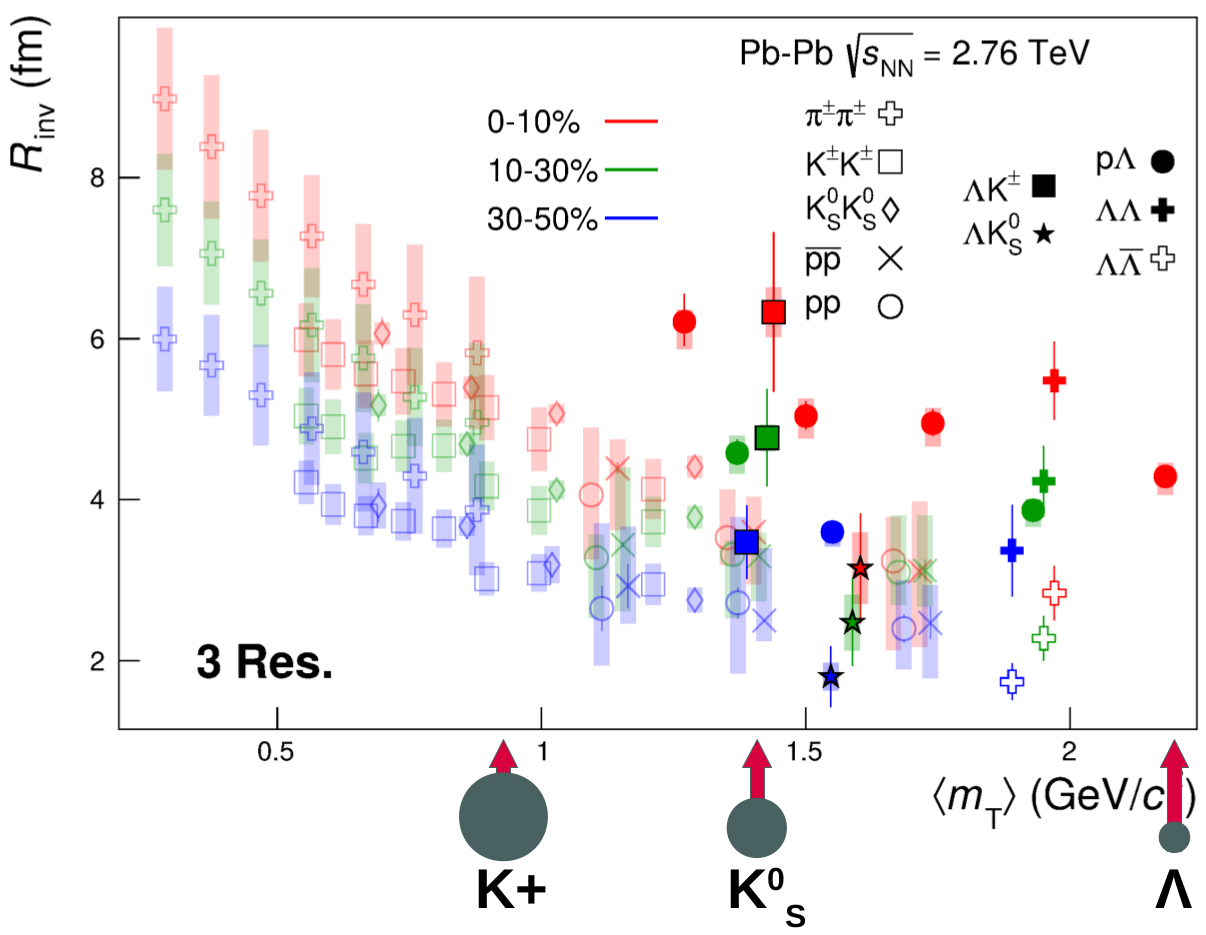
\includegraphics[width=0.75\textwidth]{/home/jesse/Analysis/FemtoAnalysis/AnalysisNotes/7_ResultsAndDiscussion/7.1_ResultsLamK/7.1.2_ResultsLamK_DiscussionOfmTScaling/OtherFigures/mTScalingwIndmTCartoon.png}
  \caption[$m_{\mathrm{T}}$ scaling of radii with individual \mt highlighted]{Same as Fig. \ref{fig:mTScalingOfRadii_3Res}, but with the individual \mt values for the single particle distributions identified.  The grey circles show how the single particle sizes are expected to change with \mt.}
  \label{fig:mTScalingOfRadii_3ReswIndmTCartoon}
\end{figure}

Taking a close look at Fig. \ref{fig:mTScalingOfRadii_3ReswIndmTCartoon}, one can see that the previously published data (transparent points) are for identical particle analyses only.
For these cases, the pair source, probed through femtoscopy, is comprised of two identical sources laying on top of each other.
The extracted femtoscopic radii are related to the single particle source sizes by a factor of $\sqrt{2}$, and of course follow the \mt-scaling trend.
The other (unpublished) non-identical particle femtoscopic study (p\Lam) included in the figure, also shows radii deviating from the \mt-scaling band.
Drawing a comparison with the $\Lambda\bar{\Lambda}$ study shown in Fig. \ref{fig:mTScalingOfRadii_3ReswIndmTCartoon} is a bit more complicated; the $\Lambda\bar{\Lambda}$ system, although containing non-identical particles, does contain a particle with its antiparticle, for which annihilation could conceivably alter the pair source distribution.
In any case, the pair source \mt-scaling visible in the identical particle femtoscopic studies presented in Fig. \ref{fig:mTScalingOfRadii_3ReswIndmTCartoon} is really just a manifestation of the scaling of the single particle sources.
For the case presented here, sampling single particle distributions with significantly different \mt values translates to sampling distributions differing in size which are separated in space-time. 
Therefore, our results deviating from the \mt-scaling curve of the identical particle studies is not surprising.

We can use Fig. \ref{fig:mTScalingOfRadii_3ReswIndmTCartoon} to estimate the values of our \LamK radii in the absence of any $\mu_{\mathrm{out}}$ offset.
As previously stated, for identical particle studies, the single particle radii can be obtained from the extracted femtoscopic radii simply by dividing by $\sqrt{2}$. 
Using the trends shown in Fig. \ref{fig:mTScalingOfRadii_3ReswIndmTCartoon}, for the \mt values appropriate for our studies, we expect the single particle source sizes in the 0-10\% centrality bin to be $R_{\mathrm{K}} \sim$ 5/$\sqrt{2}$ fm and $R_{\Lambda} \sim$ 3/$\sqrt{2}$ fm.
In Eq. \ref{eqn:PairGaussSourceWithShift} from Sec. \ref{ModelLambdaKaon}, we found the pair source radius was the sum of the single source radii added in quadrature, $R_{ab, i}^{2} = R_{a, i}^{2} + R_{b, i}^{2}$.
Therefore, we would expect $R_{\Lambda\mathrm{K}} \sim$ 4 fm, which is clearly below the value we measure.
We argue that our larger extracted radii result from a non-zero $\mu_{\mathrm{out}}$ in the pair source distribution, due to the fact that the single particle \Lam and K sources are separated in space-time.
In the following sections, we use simulation (a numerical integration method of the Koonin-Pratt equation, and THERMINATOR 2) to demonstrate the effect on one-dimensional source sizes from non-zero offsets in the ``out" direction.
Furthermore, we use a spherical harmonic decomposition of our experimental correlation functions to demonstrate that the data are consistent with a non-zero $\mu_{\mathrm{out}}$.

We emphasize that we do not suggest our extracted source sizes indicate any sort of contradiction to the hydrodynamic picture of the system dictating the substructure of the femtoscopic radii.
In fact, our results rather support such a picture.
The hydrodynamic response of the system not only confines higher-\mt particles to smaller homogeneity regions, it also pushes their average emissions points further in the ``out" direction \cite{Retiere:2003kf}.
As introduced above, these effects can lead to larger extracted radii when studying non-identical particle pairs under the assumption of a spherically symmetric Gaussian source with no offset in the ``out" direction.
This point is further supported with our numerical integration method of the Koonin-Pratt equation (presented below), as well as with our study varying $\mu_{\mathrm{out}}$ within the THERMINATOR 2 simulation (presented as the end of this section).

In summary, due to the hydrodynamic response of the system created in heavy-ion collisions, we expect higher-\mt particles to originate from smaller regions of homogeneity located further in the ``out" direction.
This difference in single particle source sizes, in addition to their separation in space-time, can lead to a deviation of non-identical particle studies from the \mt-scaling trend observed for identical particle pairs.
This is not in contradiction to the hydrodynamic response of the system, but rather in support of it.
For non-identical particle studies, the individual particle \mt values dictate the single particle source sizes and positions, which in turn dictate the observed femtoscopic signal.
Therefore, when reporting results from non-identical studies, it is vital to report the individual particle \mt values, otherwise, comparisons to other measurements will be impossible.


\paragraph*{Numerical integration of the Koonin-Pratt equation}
We investigated the effect of a non-zero offset in the outward direction, $\mu_{out}$, by numerically integrating the Koonin-Pratt equation (Eq. \ref{eqn:KooninPrattEqn}), a demonstration of which is shown in Figures \ref{fig:NumInt_LamKchP} and \ref{fig:NumInt_LamKchM}.
Before going into the details, we find that increasing $\mu_{\mathrm{out}}$ leads to a correlation function which is more tightly confined to low-\kstar values, i.e. the increase in $\mu_{\mathrm{out}}$ makes the source appear larger.
The nice analytic form for generating fit correlation functions derived by Lednick\'y relies on a spherically symmetric source distribution centered at the origin.
Using instead the method of numerical integration allows us to alter the source as we wish, which, in this case, amounts to simply adding an outward shift, $\mu_{\mathrm{out}}$, to the spherically symmetric Gaussian profile.
The cost of this flexibility is a significant decrease in the speed of generating fit curves, and this numerical integration is currently too slow to be used within our fit framework.
Nonetheless, the numerical integration method does offer a simple test ground for us to study the effect of a non-zero $\mu_{\mathrm{out}}$.

For the curves presented in Figs. \ref{fig:NumInt_LamKchP} and \ref{fig:NumInt_LamKchM}, a spherically symmetric Gaussian source ($R_{o}=R_{s}=R_{l}$) was assumed, and the offset in the ``out" direction ($\mu_{\mathrm{out}}$) was varied.
In our numerical integration, we used the appropriate forms of the wave-function and scattering parameters (Eqns. \ref{eqn:TempEq1}-\ref{eqn:PhiP1P2SphericalWave}), which were presented in Sec. \ref{ModelLambdaKaon}.
In the figure, the closed black circles show the curve generated by our numerical integrator for a radius $R_{i}$ = 6.24 fm (where $i =$ o, s, l), $\mu_{\mathrm{out}}$ = 0 fm, and the parameter sets listed in the figures ([$\Re f_{0}, \Im f_{0}, d_{0}$] = [-0.49, 0.42, -0.55] for \LamKchP in Fig. \ref{fig:NumInt_LamKchP}, and [$\Re f_{0}, \Im f_{0}, d_{0}$] = [0.19, 0.29, -7.80] for \LamKchM in Fig. \ref{fig:NumInt_LamKchM}).
Note, the radius of 6.24 fm and the parameter sets were chosen to qualitatively match the \LamKchP and \LamKchM experimental data.
The open magenta circles were generated using the analytic Lednick\'y equation (Eqns. \ref{eqn:LednickyEqn}-\ref{eqn:CFSI2} from Sec. \ref{ModelLambdaKaon}).
The figure shows that our numerical integration method is consistent with the Lednick\'y equation.
All of the triangle points assume a radius of 5 fm, again with the parameter sets listed in the legends of the figure, and the different colors correspond to different $\mu_{\mathrm{out}}$ values.

\begin{figure}[h!]
  \centering
  \includegraphics[width=\textwidth]{/home/jesse/Analysis/FemtoAnalysis/AnalysisNotes/7_ResultsAndDiscussion/7.1_ResultsLamK/7.1.2_ResultsLamK_DiscussionOfmTScaling/OtherFigures/NumIntLednickyCf_LamKchP.pdf}
  \caption[Numerical integration of Koonin-Pratt equation: \LamKchP]
  {
  Numerical integration of the Koonin-Pratt equation, allowing us to study the effect of a non-zero offset in the out direction, $\mu_{\mathrm{out}}$.
  We chose a parameter set to qualitatively match our \LamKchP data.
  The assumed scattering parameter set is printed in the top of the legend.
  All points assume $\mu_{\mathrm{side}} = \mu_{\mathrm{long}} =$ 0 fm.
  The closed black circles and open magenta symbols assume $R_{i} =$ 6.24 fm (where $i =$ o,s,l) and $\mu_{\mathrm{out}} = 0$ fm, while the triangle markers assume $R_{i} =$ 5 fm with varying values of $\mu_{\mathrm{out}}$.
  The open magenta circles were obtained with the Lednick\'y equation, all others were obtained with the numerical integration method.
  See text for more details.
  }
  \label{fig:NumInt_LamKchP}
\end{figure}

\begin{figure}[h!]
  \centering
  \includegraphics[width=\textwidth]{/home/jesse/Analysis/FemtoAnalysis/AnalysisNotes/7_ResultsAndDiscussion/7.1_ResultsLamK/7.1.2_ResultsLamK_DiscussionOfmTScaling/OtherFigures/NumIntLednickyCf_LamKchM.pdf}
  \caption[Numerical integration of Koonin-Pratt equation: \LamKchM]
  {
  Numerical integration of the Koonin-Pratt equation, allowing us to study the effect of a non-zero offset in the out direction, $\mu_{\mathrm{out}}$.
  We chose a parameter set to qualitatively match our \LamKchM data.
  The assumed scattering parameter set is printed in the top of the legend.
  All points assume $\mu_{\mathrm{side}} = \mu_{\mathrm{long}} =$ 0 fm.
  The closed black circles and open magenta symbols assume $R_{i} =$ 6.24 fm (where $i =$ o,s,l) and $\mu_{\mathrm{out}} = 0$ fm, while the triangle markers assume $R_{i} =$ 5 fm with varying values of $\mu_{\mathrm{out}}$.
  The open magenta circles were obtained with the Lednick\'y equation, all others were obtained with the numerical integration method.
  See text for more details.
  }
  \label{fig:NumInt_LamKchM}
\end{figure}


Figures \ref{fig:NumInt_LamKchP} and \ref{fig:NumInt_LamKchM} nicely demonstrate the effect of increasing the magnitude of the offset.
Specifically, the figure shows that increasing $\mu_{\mathrm{out}}$ makes the correlation function more concentrated towards the low-\kstar region, which corresponds to larger radii.
Furthermore, for a one-dimensional analysis, we see that the case of a spherically symmetric source with $R_{i}=$ 6.24 fm (where $i$ = o,s,l) is nearly indistinguishable from a source with $R_{i}=$ 5 fm and $\mu_{\mathrm{out}} =$ 8 fm.
Therefore, even with a fast numerical integrator, it would be difficult to disentangle the effects of a larger source radius from a shift in the ``out" direction.
In order to pursue this direction, outside input constraining these parameters would be necessary.
This could be accomplished, for instance,  by fixing the single particle source sizes, and therefore the pair source size, using identical KK and $\Lambda\Lambda$ results.


%%%%%%%%%%%%%%%%%%%%%%%%%%%%%%%%%%%%%%%%%%%%%%%%%%%%%%%%%%%%%%%%%%%%%%%%%%%%%%%%%%%%%%%%%%%%%%%%%%%%%%%%%%%%%%%%%%%%%%%%%%
\begin{comment}
\begin{figure}[h!]
  \centering
  %%----start of first subfigure---  
  \subfloat[\LamKchP]{
    \label{fig:NumInt:a}
    \includegraphics[width=0.75\linewidth]{/home/jesse/Analysis/FemtoAnalysis/AnalysisNotes/7_ResultsAndDiscussion/7.1_ResultsLamK/7.1.5_ResultsLamK_DiscussionOfmTScaling/OtherFigures/NumIntLednickyCf_LamKchP.pdf}} \\
  %%----start of second subfigure---
  \subfloat[\LamKchM]{
    \label{fig:NumInt:b}
    \includegraphics[width=0.75\linewidth]{/home/jesse/Analysis/FemtoAnalysis/AnalysisNotes/7_ResultsAndDiscussion/7.1_ResultsLamK/7.1.5_ResultsLamK_DiscussionOfmTScaling/OtherFigures/NumIntLednickyCf_LamKchM.pdf}}  
  %%----overall caption----
  \caption[Numerical integration for correlation function]
  {
  Numerical integration of the Koonin-Pratt equation, allowing us to study the effect of a non-zero offset in the out direction, $\mu_{\mathrm{out}}$.
  In the top, we chose a parameter set to qualitatively match our \LamKchP data, while in the bottom we match the \LamKchM system.
  The assumed scattering parameter set is printed in the top of each legend.
  All points assume $\mu_{\mathrm{side}} = \mu_{\mathrm{long}} =$ 0 fm.
  The closed black circles and open magenta symbols assuming $R_{i} =$ 6.24 fm (where $i =$ o,s,l) and $\mu_{\mathrm{out}} = 0$ fm, while the triangle markers assume $R_{i} =$ 5 fm with varying values of $\mu_{\mathrm{out}}$.
  The open magenta circles were obtained with the Lednick\'y equation, all others were obtained with the numerical integration method.
  See text for more details.
  }
  \label{fig:NumInt}
\end{figure}
\end{comment}
%%%%%%%%%%%%%%%%%%%%%%%%%%%%%%%%%%%%%%%%%%%%%%%%%%%%%%%%%%%%%%%%%%%%%%%%%%%%%%%%%%%%%%%%%%%%%%%%%%%%%%%%%%%%%%%%%%%%%%%%%%










%%%%%%%%%%%%%%%%%%%%%%%%%%%%%%%%%%%%%%%%%%%%%%%%%%%%%%%%%%%%%%%%%%%%%%%%%%%%%%%%%%%%%%%%%%%%%%%%%%%%%
\begin{comment}
I will also briefly point out that it is not automatically clear where a non-identical study should be placed on such a $R_{\mathrm{inv}}$ vs \mt plot.
Each single particle distribution has a well-defined $\langle m_{\mathrm{T}} \rangle$, which, to a large extent, determines the single particle region of homogeneity.
When combining two sources with different spatio-temporal characteristics, originating from particles of different \mt, how should one define the pair \mt?
A simple mathematical expression for the pair \mt is easy to come up with, but that's not exactly what I'm hinting at here.
With respect to this \mt-scaling picture, the \mt value dictates the source size, and one desires the same for non-identical particles.
However, do the two unequal sized sources both contribute equally to the extracted femtoscopic size?
Or does the larger (smaller) source more closely dictate the femtoscopic signal?
If the contribution is equal, then it seems natural to simply more-or-less average the two, single particle, \mt values.
If the contribution is unequal, then there should be introduced some sore of weighting in the pair \mt calculation reflecting this fact.
In any case, in our study we use the most straightforward definition of pair \mt, defined as:


\begin{equation}
 m_{\mathrm{T, pair}}^{2} = \left( \frac{m_{\mathrm{inv}}}{2} \right)^{2} + \left( \frac{1}{2} |\textbf{\textit{p}}_{\mathrm{T,1}} + \textbf{\textit{p}}_{\mathrm{T,2}}| \right)^{2}
\label{eqn:PairmTv1}
\end{equation}

Many times, the equation for non-identical particle pair \mt is defined with the average mass replacing $m_{\mathrm{inv}}/2$.  However, the above Eq. \ref{eqn:PairmTv1} is more directly analogous to the single particle \mt:

\begin{equation}
 m_{\mathrm{T}}^{2} = m^{2} + \textbf{\textit{p}}_{\mathrm{T}}^{2} = (p^{0})^{2} - (p^{3})^{2}
\label{eqn:SinglemT}
\end{equation}

as, Eq. \ref{eqn:PairmTv1} may be rewritten as:



\begin{equation}
\begin{aligned}
m_{\mathrm{T, pair}}^{2} &= (K^{0})^{2} - (K^{3})^{2} \\
K^{\mu} & \equiv \frac{1}{2} \left( p_{1}^{\mu} + p_{2}^{\mu} \right)
\end{aligned}
\label{eqn:PairmTv2}
\end{equation}
\end{comment}
%%%%%%%%%%%%%%%%%%%%%%%%%%%%%%%%%%%%%%%%%%%%%%%%%%%%%%%%%%%%%%%%%%%%%%%%%%%%%%%%%%%%%%%%%%%%%%%%%%%%%

\paragraph*{Spherical harmonics and varying $\mu_{\mathrm{out}}$ with THERMINATOR 2}

Identical particle femtoscopic studies are able to probe only the size of the emitting region, or, more precisely, the second moments of the emission function.
In addition to this, non-identical particle studies are able to measure the relative emission shifts, the first moments of the emission function.
One method to extract information about the emission asymmetries in the system is via a spherical decomposition of the correlation function.
With this method, one can draw a wealth of information from just a few components of the decomposition.
More specifically, the $C_{00}$ component is similar to the 1D correlation functions typically studied, and probes the overall size of the source.
The $\Re C_{11}$ component probes the asymmetry in the system; a non-zero value reveals the asymmetry. 

In Fig. \ref{fig:LamKchP_ReC00C11_0010} we show results for the $C_{00}$ and $\Re C_{11}$ components from the spherical decomposition of our \LamKchP system in the 0-10\% centrality bin (red circles).
Results from a number of other components within the decomposition, as well as for our \LamKs and \LamKchM systems, are contained in App. \ref{Appendix_SphericalHarmonics}.
Along with the experimental data in Fig. \ref{fig:LamKchP_ReC00C11_0010}, we have also included results from THERMINATOR simulation for an impact parameter of b = 2 fm (gold stars).
As THERMINATOR does not include any final state effects, we assumed scattering parameters ($\Re f_{0}, \Im f_{0}, d_{0}$) = (-1.16, 0.51, 1.08) and weighted the numerator pairs with $|\Psi|^{2}$, as discussed previously in Sec. \ref{NonFlatBackground} (with regard to Fig. \ref{fig:THERMCfBgdDecomposition}).
Note, for the \LamKchP system, THERMINATOR 2 predicts $\mu_{\mathrm{out}} \approx$ 4 fm, as shown in Fig. \ref{fig:LamKchP_StdThermSources} 
As seen in the figures, the $C_{00}$ signal is similar to that observed in our one-dimensional study.
The $\Re C_{11}$ component shows a clear deviation from zero, and the negative value signifies that the \Lam particles are, on average, emitted further out and/or earlier than the K mesons (in defining our pairs, we take the heavier \Lam as our first particle, which is opposite the normal convention).
Therefore, as expected, our single particle \Lam and K sources are separated in space-time.

\begin{figure}[h!]
  \centering
  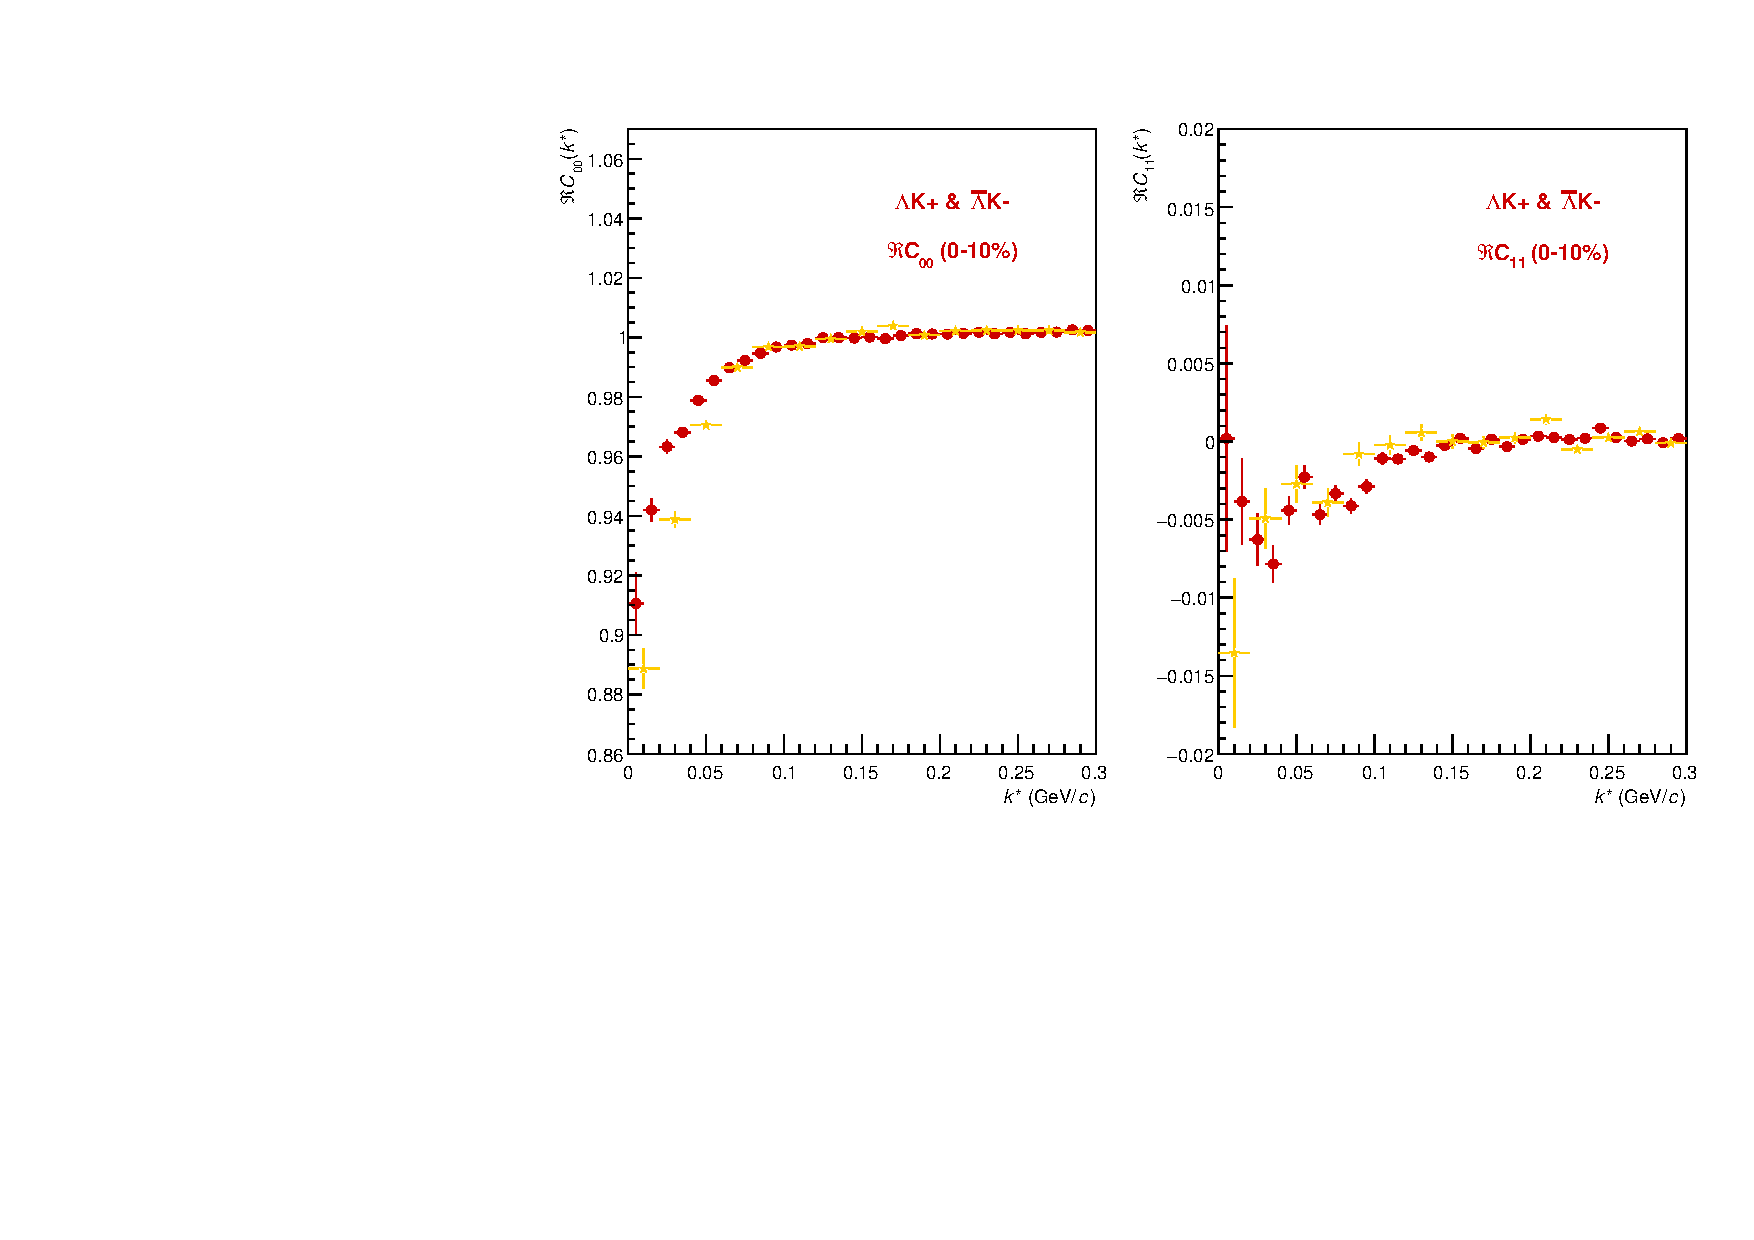
\includegraphics[width=\textwidth]{\ResultsDirBase Results_cLamcKch_20181205/SphericalHarmonics/LamKchP/CanCfYlmReC00C11_LamKchPALamKchM_0010_wTherm.pdf}
  \caption[\LamKchP $C_{00}$ and $\Re C_{11}$ spherical harmonic components (0-10\%)]{$C_{00}$ (left) and $\Re C_{11}$ (right) components of a spherical harmonic decomposition of the \LamKchP correlation function for the 0-10\% centrality bin.  
The $C_{00}$ component is similar to the 1D correlation functions typically studied, and probes the overall size of the source.
The $\Re C_{11}$ component probes the asymmetry in the system; a non-zero value reveals the asymmetry}
  \label{fig:LamKchP_ReC00C11_0010}
\end{figure}


Fig. \ref{fig:LamKchP_StdThermSources} shows a closer look at the THERMINATOR simulation, whose spherical harmonic decomposition was shown along with the data in Fig. \ref{fig:LamKchP_ReC00C11_0010}.
The top left of Fig. \ref{fig:LamKchP_StdThermSources_Spatial} shows a fit to the one-dimensional correlation function from THERMINATOR.
The scattering parameters are known precisely here, as they served as the weights used in the simulation, and are kept constant in the fit.
We are interested at looking at the extracted one-dimensional source size here, so the $\lambda$ parameter is also fixed at unity.
The other three plots in Fig. \ref{fig:LamKchP_StdThermSources_Spatial} show the source distribution in the out (top right), side (bottom left), and long (bottom right) directions (all in the PRF).
The source distributions have all been fitted with a Gaussian form, the result of which is printed within the respective plots.
One immediately sees a significant shift in the out direction, $\mu_{\mathrm{out}} \approx$ 4 fm, and negligible shift in the other two directions, $\mu_{\mathrm{side}} \approx \mu_{\mathrm{long}} \approx$ 0 fm.
The figure demonstrates that, within the THERMINATOR model, the \Lam is, on average, emitted further out that its K partner.
Finally, Fig. \ref{fig:LamKchP_StdThermSources_Temporal} shows the distribution of the relative time of emittance, again in the PRF.
The figure shows that the \Lam is, on average, emitted earlier than its K partner.
These two results from THERMINATOR 2 are as expected.


\begin{figure}[h!]
  \centering
  %%----start of first subfigure---  
  \subfloat[(Top Left) Simple fit on simulation from THERMINATOR 2. Generated source in the (Top Right) out, (Bottom Left) side, and (Bottom Right) long directions.]{
    \label{fig:LamKchP_StdThermSources_Spatial}
    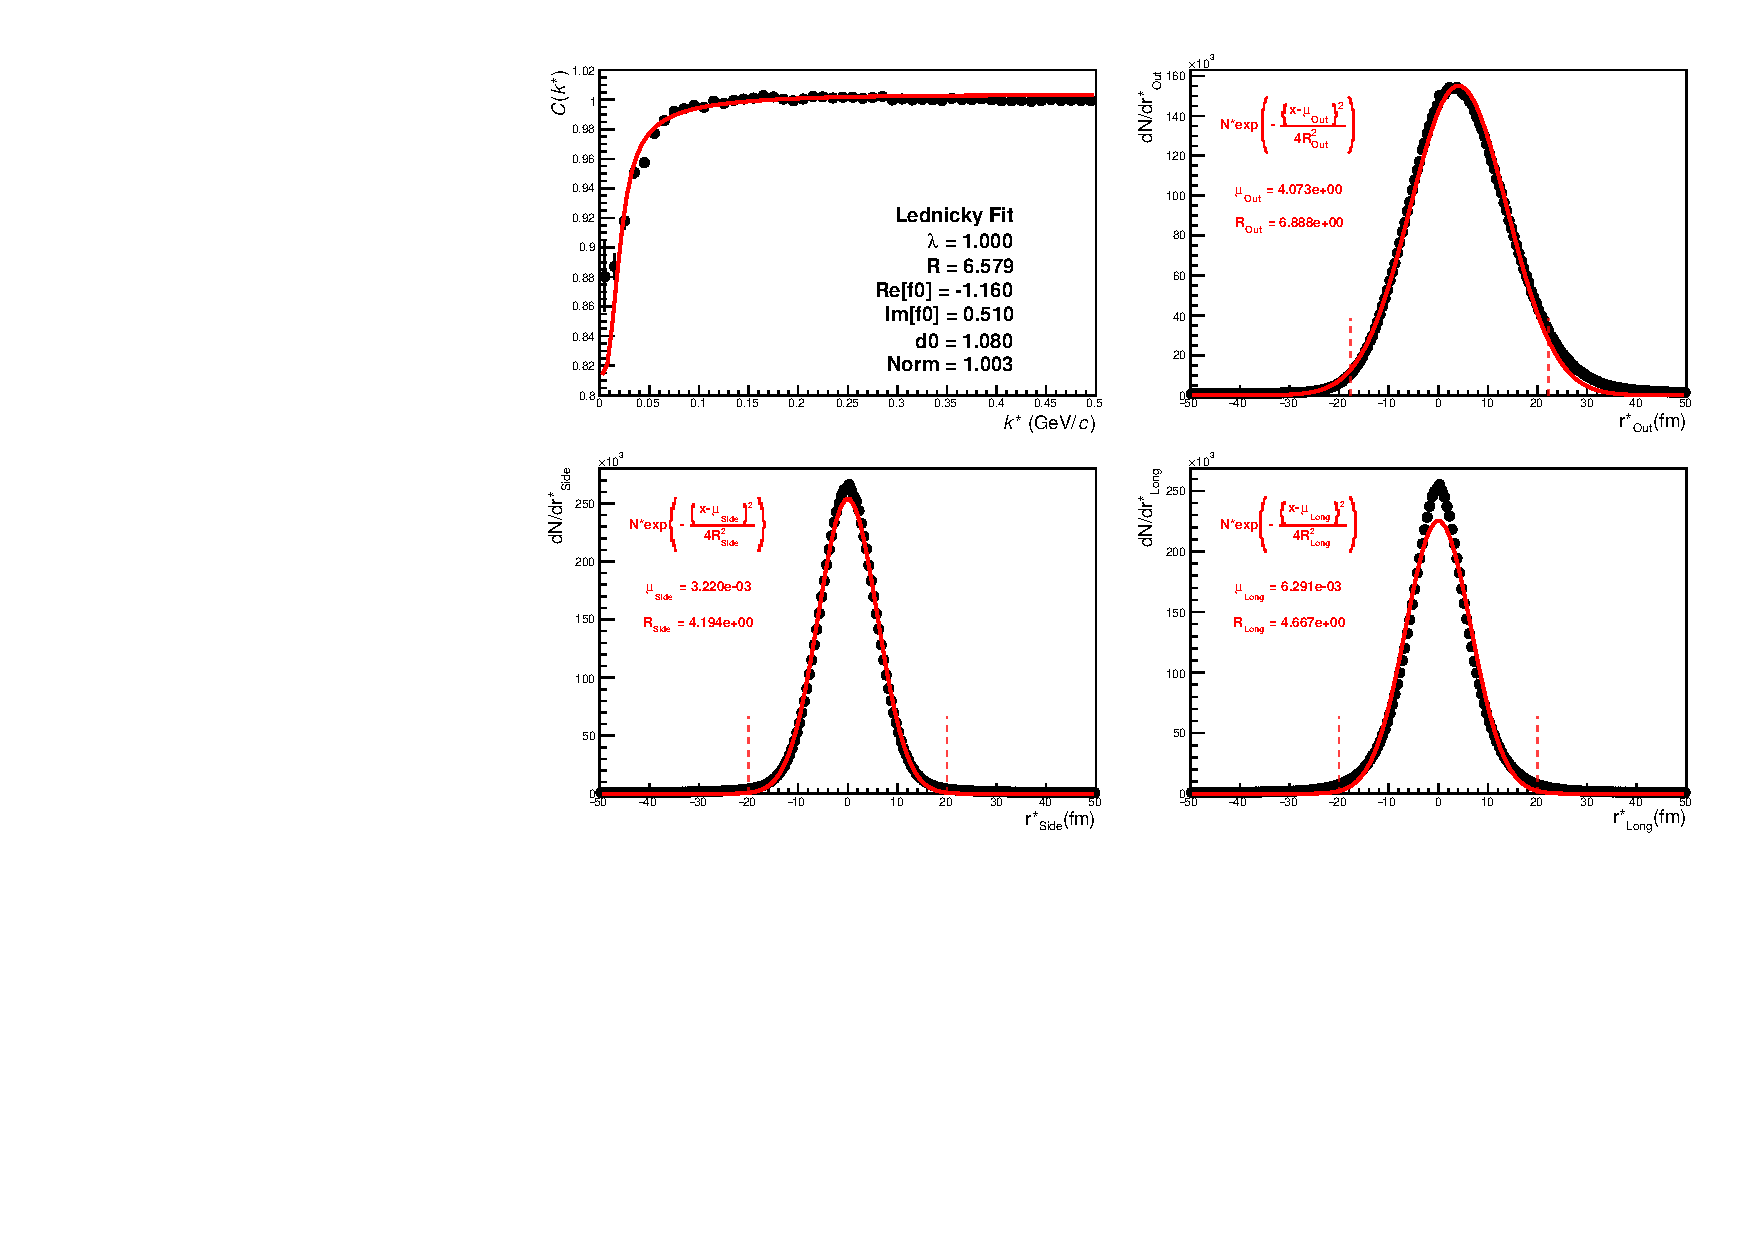
\includegraphics[width=\linewidth]{/home/jesse/Analysis/FemtoAnalysis/AnalysisNotes/7_ResultsAndDiscussion/7.1_ResultsLamK/7.1.2_ResultsLamK_DiscussionOfmTScaling/ThermPlots/LamKchP/CanCfwSource_Full_LamKchP_3dHistPairSource3d_oslLamKchP_FromFileCorrelationFunctions_wOtherPairs.pdf}} \\
  %%----start of second subfigure---
  \subfloat[Temporal characteristics of the source.]{
    \label{fig:LamKchP_StdThermSources_Temporal}
    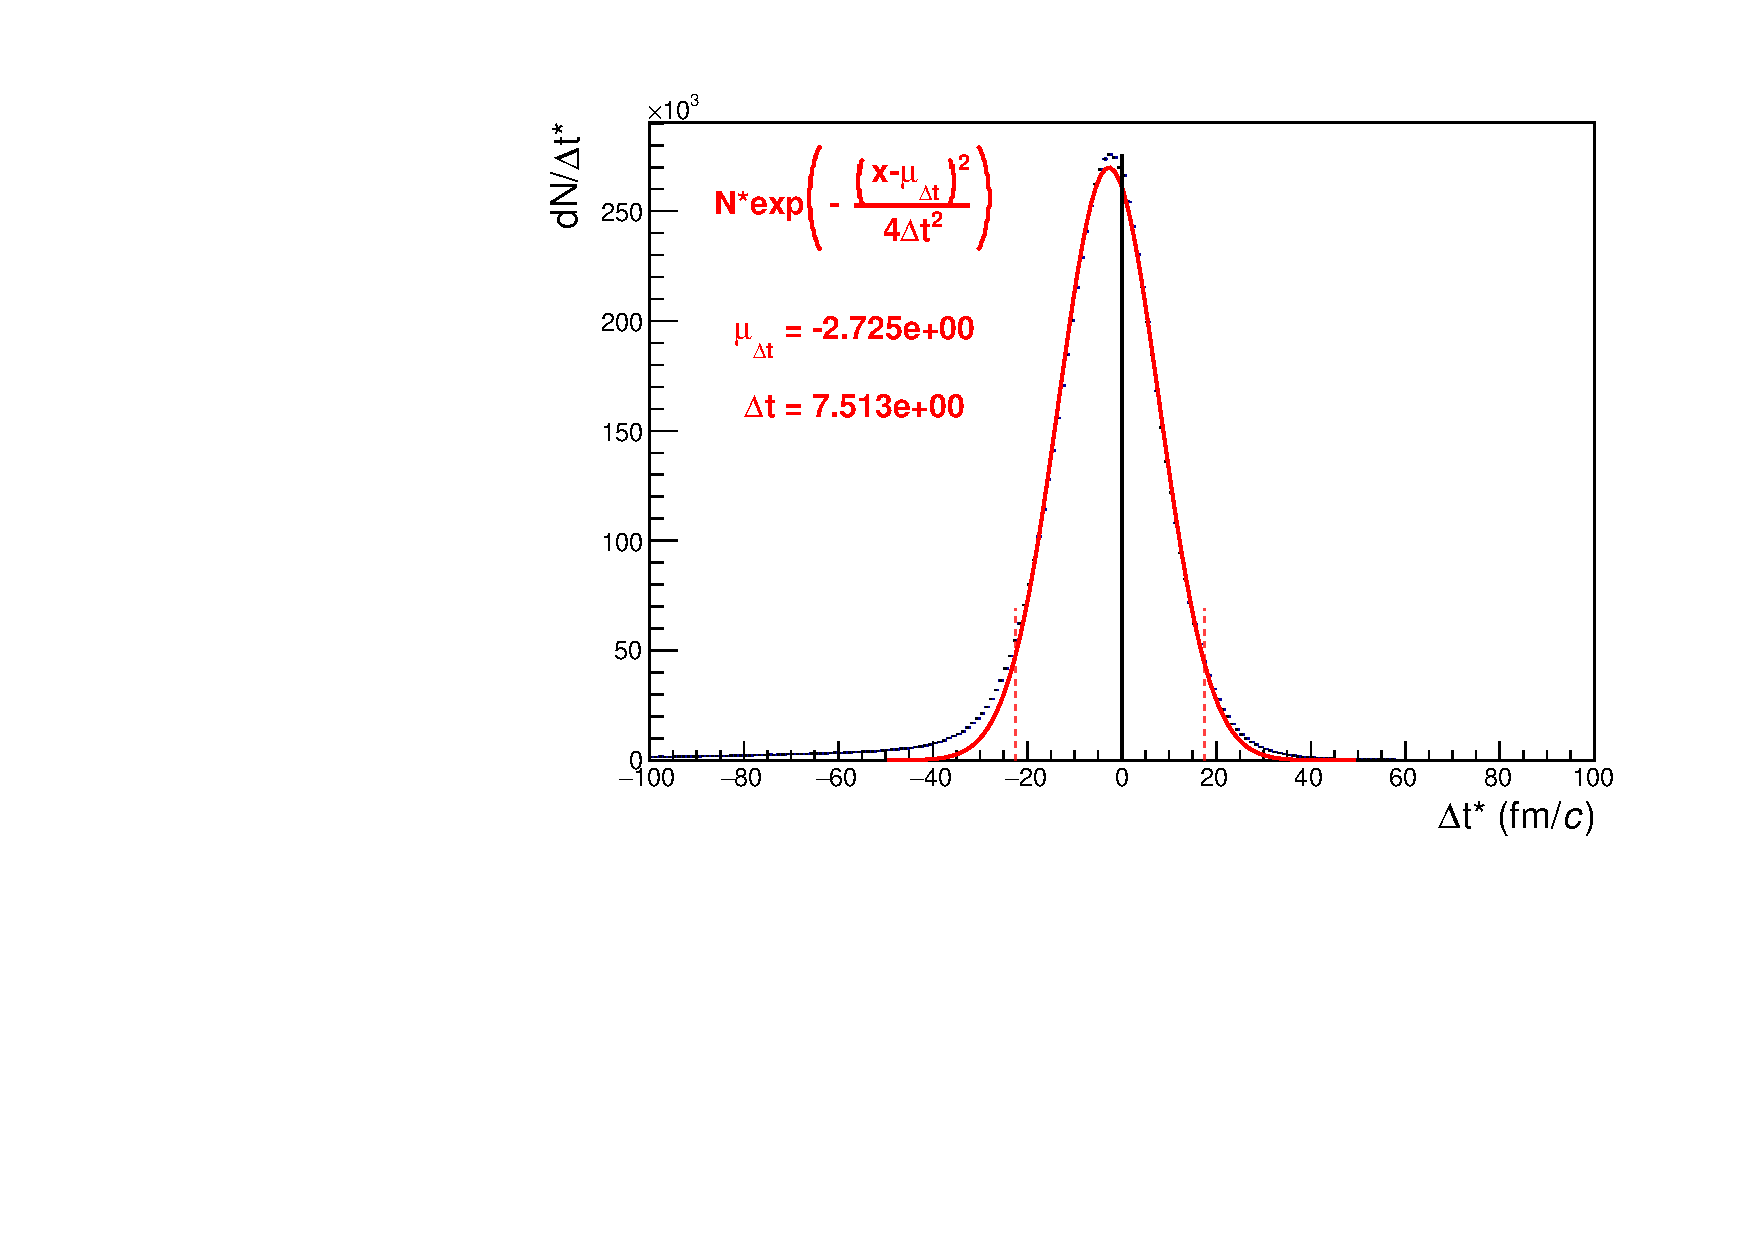
\includegraphics[width=0.60\linewidth]{/home/jesse/Analysis/FemtoAnalysis/AnalysisNotes/7_ResultsAndDiscussion/7.1_ResultsLamK/7.1.2_ResultsLamK_DiscussionOfmTScaling/ThermPlots/LamKchP/CanDeltaT_Full_LamKchP_FromFileCorrelationFunctions_wOtherPairs_BuildCfYlm.pdf}}  
  %%----overall caption----
  \caption[Extracted radius with pair sources from THERMINATOR 2]{Extracted radius when performing a simple fit on simulation from THERMINATOR 2, along with the spatio-temporal characteristics generated by the simulation.}
  \label{fig:LamKchP_StdThermSources}
\end{figure}




We end this section with a brief look at how a spatial separation of the single particle sources affects the radii extracted from a femtoscopic analysis.
To achieve this, we use THERMINATOR in a similar fashion as described above, but with one important difference.
Instead of taking the source information from THERMINATOR, we draw the source from pre-determined Gaussian distributions.
In all cases, we take $R_{\mathrm{out}} = R_{\mathrm{side}} = R_{\mathrm{long}}$ = 5 fm, and $\mu_{\mathrm{side}} = \mu_{\mathrm{long}}$ = 0 fm.
Figure \ref{fig:LamKchP_ThermSources_GaussianSourceEx} shows an example of results obtained from THERMINATOR following this procedure, where $\mu_{\mathrm{out}}$ = 3 fm.


\begin{figure}[h]
  \centering
  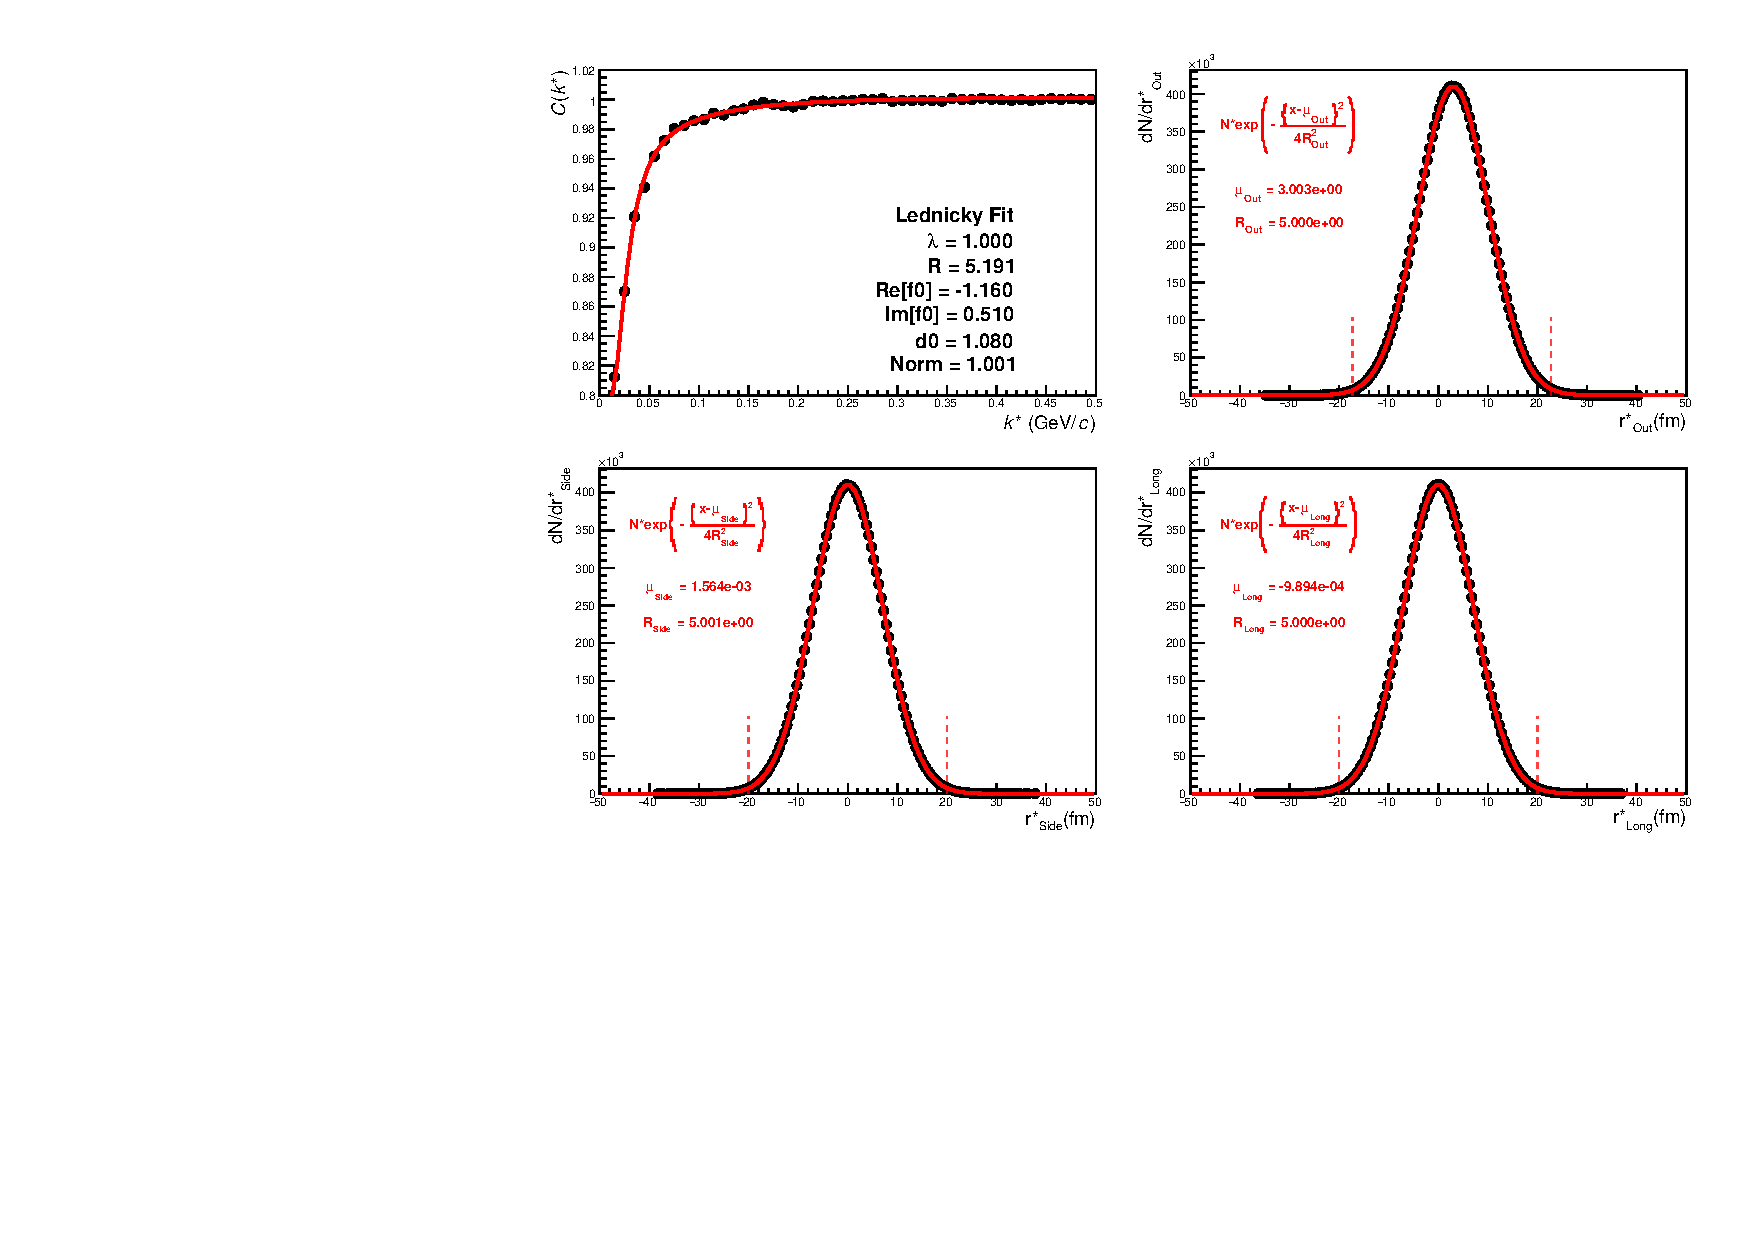
\includegraphics[width=\textwidth]{/home/jesse/Analysis/FemtoAnalysis/AnalysisNotes/7_ResultsAndDiscussion/7.1_ResultsLamK/7.1.2_ResultsLamK_DiscussionOfmTScaling/ThermPlots/LamKchP/CanCfwSource_Full_LamKchP_3dHistPairSource3d_oslLamKchP_FromFileCorrelationFunctions_wOtherPairs_DrawRStarFromGaussian_BuildCfYlm_cLamcKchMuOut3_cLamK0MuOut3_KchPKchPR538.pdf}
  \caption[THERMINATOR 2 simulation with artificial Gaussian source]
  {
  THERMINATOR 2 simulation with artificial Gaussian source.
  The figure shows the extracted radius when performing a simple fit on simulation from THERMINATOR 2 (similar to Fig. \ref{fig:LamKchP_StdThermSources_Spatial}), except the space-time information provided by the simulation is ignored.
  Instead, the components of the spatial separation for each pair were drawn from Gaussian distributions, with $\sigma^{2}_{o,s,l} = 5$ fm, $\mu_{s,l} = 0$ fm, and $\mu_{o} = 3$ fm.
  The separation of emission in time was taken to be zero.
  (Top Left) Simple fit on simulation from THERMINATOR 2. 
  Source in the (Top Right) out, (Bottom Left) side, and (Bottom Right) long directions.
  }
  \label{fig:LamKchP_ThermSources_GaussianSourceEx}
\end{figure}


In Figure \ref{fig:LamKchP_ThermSources_VaryMuOut}, we show results for the case of $\mu_{out}$ = 1 fm, $\mu_{out}$ = 3 fm, and $\mu_{out}$ = 6 fm.
In this figure, we do not show the side and long distributions, as they appear identical to those shown in Fig. \ref{fig:LamKchP_ThermSources_GaussianSourceEx}.
The figure demonstrates that as the separation $\mu_{out}$ increases, so do the extracted femtoscopic radii.
This is exactly as expected, and in agreement with our qualitative assessment of the curves generated by our numerical Koonin-Pratt integrator described above.


\begin{figure}[h]
  \centering
  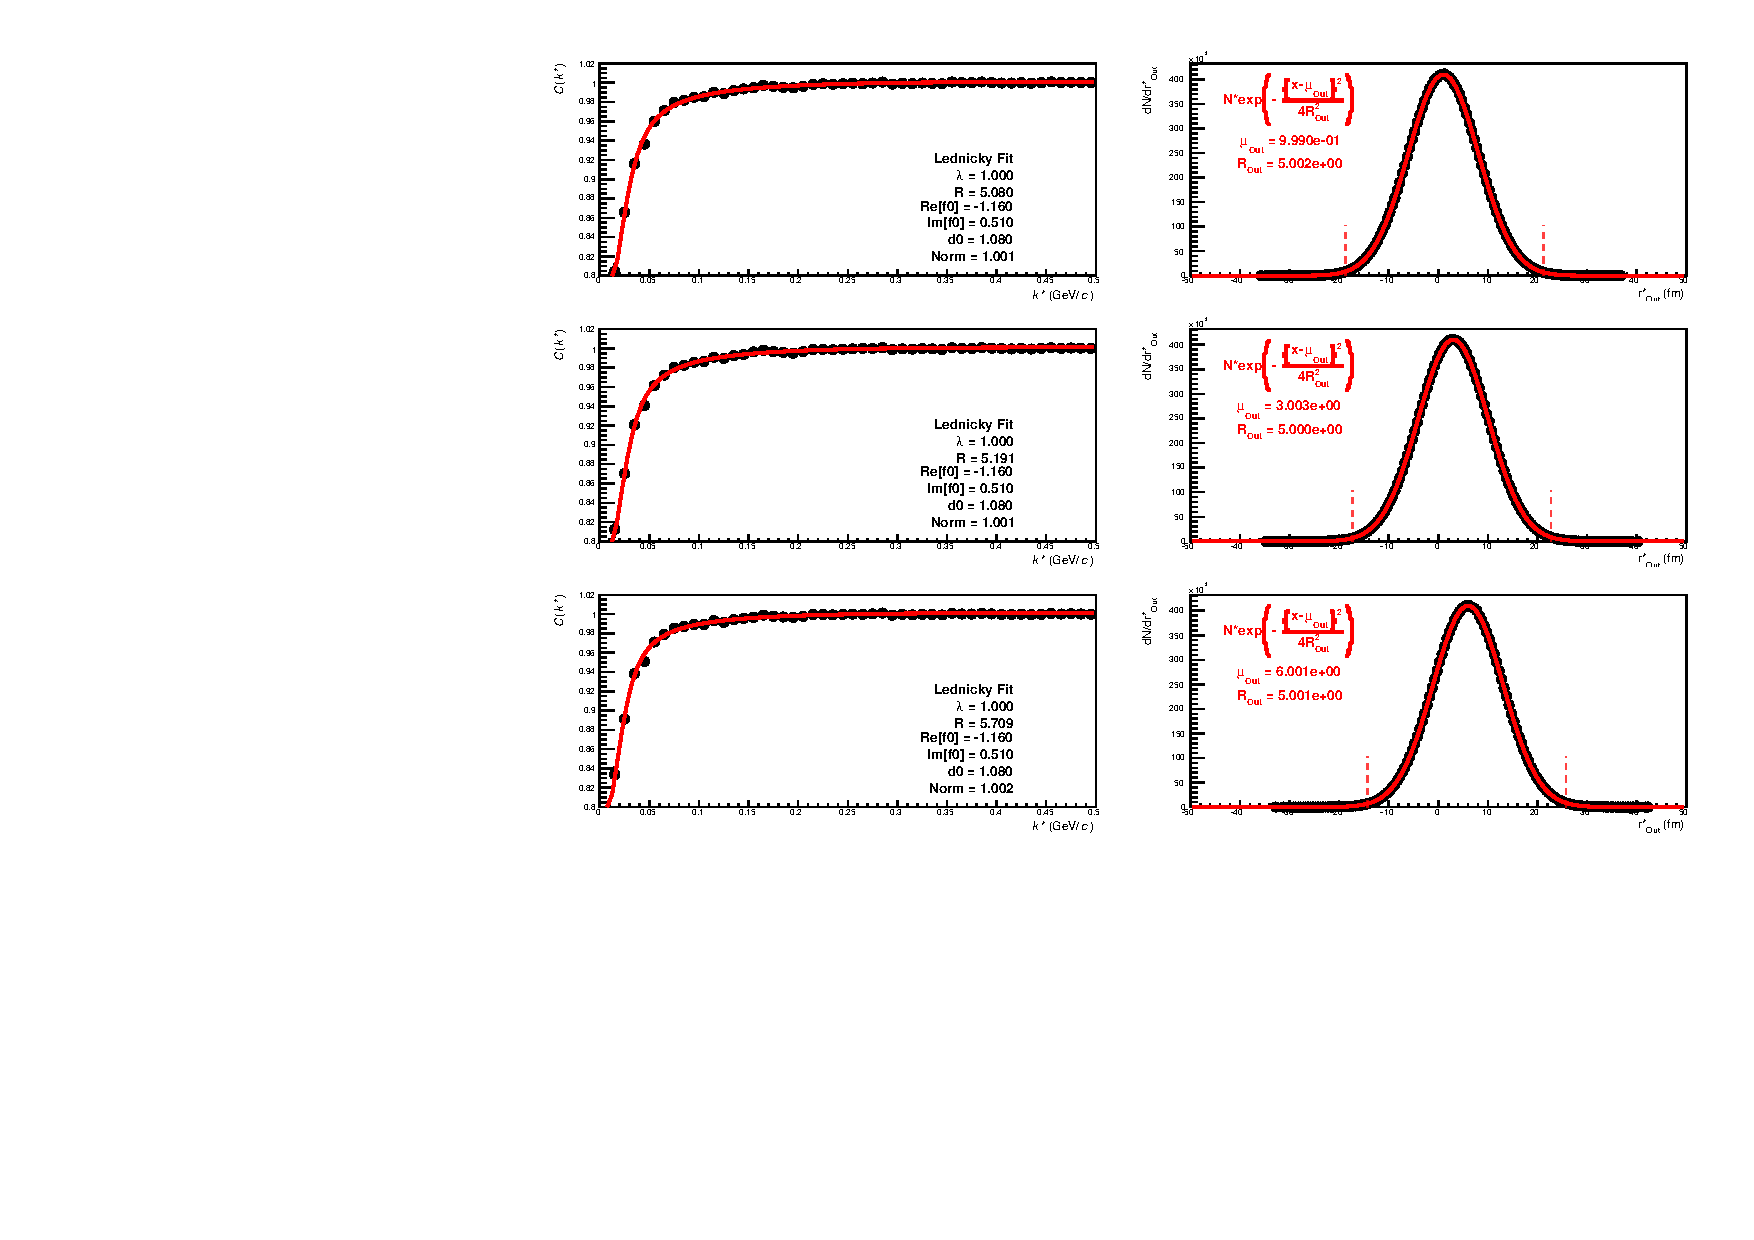
\includegraphics[width=\textwidth]{/home/jesse/Analysis/FemtoAnalysis/AnalysisNotes/7_ResultsAndDiscussion/7.1_ResultsLamK/7.1.2_ResultsLamK_DiscussionOfmTScaling/ThermPlots/LamKchP/CanCompMus_Full_LamKchP_3dHistPairSource3d_oslLamKchP.pdf}
  \caption[Varying $\mu_{\mathrm{Out}}$ with THERMINATOR 2]{Probing the effect of varying the source shift in the outward direction, $\mu_{\mathrm{Out}}$, within the THERMINATOR 2 framework.  To achieve this, we formed particle pairs from the simulation, but altered their spatial characteristics by drawing the out, side, and long components from pre-determined Gaussian distributions.  The plots on the left show fits resulting from the sources (in the out direction) shown on the right.  The sources in the side and long directions are not shown, and are both Gaussians of width 5 fm centered at the origin for all cases.  Moving from top to bottom, $\mu_{\mathrm{Out}}$ increase from 0 to 6 fm, the effect of which clearly increases the effective radius extracted in the fit.}
  \label{fig:LamKchP_ThermSources_VaryMuOut}
\end{figure}


\paragraph*{Comparing non-identical to identical particle result}
Non-identical femtoscopic analyses are not so simply compared to identical particle studies.
However, a method was presented in which the single particle source sizes can be extracted using three related femtoscopic measurements, which can then be related to the results from identical particle studies \cite{Kisiel:2009eh}.
Extracting the single particle source size from and identical study simply amounts to dividing the extracted radii by $\sqrt{2}$.
For non-identical studies, the procedure is not so simple.
As introduced in Sec. \ref{ModelLambdaKaon}, assuming the single particle sources are three dimensional Gaussians with offsets in the ``out" direction, the pair source distribution is also a Gaussian with offset in the ``out" direction.
The form of the Gaussian is given in Eq. \ref{eqn:PairGaussSourceWithShift}, and reproduced here for convenience.
\begin{equation}
\begin{aligned}
S_{AB}(\mathbf{r}) &\propto \exp\left(-\frac{[r_{out}-(\mu_{a, out}-\mu_{b, out})]^{2}}{2(R_{a,out}^{2}+R_{b,out}^{2})}\right) \times ... \\
&~~~~\times \exp\left(-\frac{r_{side}^{2}}{2(R_{a,side}^{2}+R_{b,side}^{2})}\right) \times ... \\
&~~~~\times \exp\left(-\frac{r_{long}^{2}}{2(R_{a,long}^{2}+R_{b,long}^{2})}\right)
\end{aligned}
\label{eqn:PairGaussSourceWithShiftv2}
\end{equation}
which demonstrates $\mu_{ab, out} = \mu_{a, out}-\mu_{b, out}$, and $R_{ab, i}^{2} = R_{a, i}^{2} + R_{b, i}^{2}$.
Unfortunately, with a single femtoscopic measurement, the two single particle source sizes cannot be extracted.
However, in Ref. \cite{Kisiel:2009eh}, the author demonstrated that using three related femtoscopic measurements, the single particle sizes can be extracted.
However, this method does rely on including $\mu_{\mathrm{out}}$ in the fit.

Performing measurements of the systems $\pi\mathrm{K}$, $\pi\mathrm{p}$ and $\mathrm{K}\mathrm{p}$ permits one to extract the single particle $\pi$, K, and p source sizes.
In Ref. \cite{Kisiel:2009eh}, the author assumed $R_{\mathrm{out}} = R_{\mathrm{side}} = \sigma_{f}$, $R_{\mathrm{long}} = 1.3\sigma_{f}$ and $\mu_{\mathrm{side}} = \mu_{\mathrm{long}} = 0$.
Furthermore, having reliable estimates of the scattering parameters for the systems, only two fit parameters, $R_{\mathrm{out}}$ and $\mu_{\mathrm{out}}$ were left, and easily extracted.
Given the fact that $R_{ab, i}^{2} = R_{a, i}^{2} + R_{b, i}^{2}$, for the three systems we therefore have
\begin{equation}
\begin{aligned}
\sigma_{f}^{\pi\mathrm{K}} = \sqrt{{\sigma_{f}^{\pi}}^{2} + {\sigma_{f}^{\mathrm{K}}}^{2}} \\
\sigma_{f}^{\pi\mathrm{p}} = \sqrt{{\sigma_{f}^{\pi}}^{2} + {\sigma_{f}^{\mathrm{p}}}^{2}} \\
\sigma_{f}^{\mathrm{K}\mathrm{p}} = \sqrt{{\sigma_{f}^{\mathrm{K}}}^{2} + {\sigma_{f}^{\mathrm{p}}}^{2}} 
\label{eqn:PiKPEqns1}
\end{aligned}
\end{equation}
These three equations can then be solved for the single particle source sizes
\begin{equation}
\begin{aligned}
\sigma_{f}^{\pi} = \sqrt{\left({\sigma_{f}^{\pi\mathrm{K}}}^{2} + {\sigma_{f}^{\pi\mathrm{p}}}^{2} - {\sigma_{f}^{\mathrm{K}\mathrm{p}}}^{2}\right)/2} \\
\sigma_{f}^{\mathrm{K}} = \sqrt{\left({\sigma_{f}^{\pi\mathrm{K}}}^{2} - {\sigma_{f}^{\pi\mathrm{p}}}^{2} + {\sigma_{f}^{\mathrm{K}\mathrm{p}}}^{2}\right)/2} \\
\sigma_{f}^{\mathrm{p}} = \sqrt{\left({-\sigma_{f}^{\pi\mathrm{K}}}^{2} + {\sigma_{f}^{\pi\mathrm{p}}}^{2} + {\sigma_{f}^{\mathrm{K}\mathrm{p}}}^{2}\right)/2} \\
\label{eqn:PiKPEqns2}
\end{aligned}
\end{equation}
These extracted single particle source sizes can then be compared to those obtained using identical particle femtoscopy to check for consistency.
Unfortunately, with our analysis, we are unable to include $\mu_{\mathrm{out}}$ in our fit, and therefore are unable to utilize a similar type of solution.


\clearpage
\end{document}